\documentclass[tikz,border=10pt]{standalone}
\usepackage{amsmath}

\begin{document}
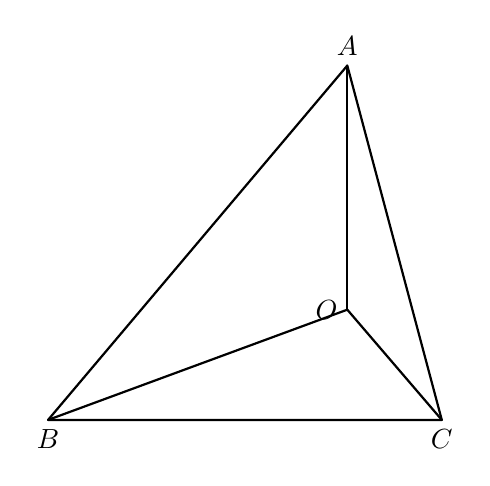
\begin{tikzpicture}[line join=round, line cap=round, >=stealth]
    % 1. 定义关键点的坐标
    % 为了符合原图视觉比例：
    % B点设为原点，BC为水平线
    \coordinate (B) at (0, 0);
    \coordinate (C) at (5, 0);
    \coordinate (A) at (3.8, 4.5); % A点较高，偏右
    \coordinate (O) at (3.8, 1.4); % O点在A正下方附近，形成类似投影的视觉

    % 2. 绘制三角形外边界 ABC
    \draw[thick] (A) -- (B) -- (C) -- cycle;

    % 3. 绘制内部连接线 OA, OB, OC
    \draw[thick] (O) -- (A);
    \draw[thick] (O) -- (B);
    \draw[thick] (O) -- (C);

    % 4. 标注顶点标签
    % 调节 label 的位置 (above, below, left, right) 以匹配原图图标
    \node[above] at (A) {$A$};
    \node[below] at (B) {$B$};
    \node[below] at (C) {$C$};
    \node[left]  at (O) {$O$};

\end{tikzpicture}
\end{document}